\documentclass{article}
\usepackage[utf8]{inputenc}
\usepackage{hyperref}
\usepackage[letterpaper, portrait, margin=1in]{geometry}
\usepackage{enumitem}
\usepackage{amsmath}
\usepackage{booktabs}
\usepackage{graphicx}

\usepackage{hyperref}
\hypersetup{
colorlinks=true,
    linkcolor=black,
    filecolor=black,      
    urlcolor=blue,
    citecolor=black,
}
\usepackage{natbib}

\usepackage{titlesec}
  
\title{HW4}
\author{Ryan Ellis}
\date{Spring semester 2023}
  
\begin{document}
  
\maketitle

\section{Python}
\subsection{}
\begin{figure}[hbt!]
    \centering
    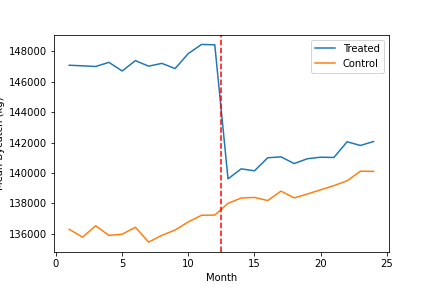
\includegraphics[scale=0.9]{homework4/output/image1.png}
    \caption{Caption}
    \label{fig:my_label}
\end{figure}

\subsection{}
\begin{itemize}
    \item The point estimate for the coefficient of interest is -9591.35. It implies that the treatment reduces bycatch by that amount, in pounds. 
\end{itemize}

\clearpage
\subsection{}

\begin{table}[hbt!] \centering
\begin{table}[!htbp] \centering
\begin{tabular}{@{\extracolsep{5pt}}lccc}
\\[-1.8ex]\hline
\hline \\[-1.8ex]
& \multicolumn{3}{c}{\textit{Dependent variable:}} \
\cr \cline{3-4}
\\[-1.8ex] & (1) & (2) & (3) \\
\hline \\[-1.8ex]
 const & 137228.60$^{***}$ & 136154.05$^{***}$ & 1547.01$^{***}$ \\
  & (18543.61) & (12035.83) & (346.41) \\
 Firm Size & & & -2119.71$^{**}$ \\
  & & & (982.42) \\
 Pre-treatment & 773.22$^{}$ & & \\
  & (26238.57) & & \\
 Salmon & & & 0.60$^{***}$ \\
  & & & (0.06) \\
 Shrimp & & & 1.06$^{***}$ \\
  & & & (0.02) \\
 Treated & -9591.35$^{}$ & -8956.78$^{}$ & -8436.28$^{***}$ \\
  & (33094.88) & (9435.06) & (806.64) \\
 Treatment Group & 11202.04$^{}$ & 11052.45$^{*}$ & -21.90$^{}$ \\
  & (23383.90) & (6624.65) & (94.15) \\
\hline \\[-1.8ex]
 Observations & 100 & 1,200 & 1,200 \\
 $R^2$ & 0.00 & 0.00 & 0.99 \\
 Adjusted $R^2$ & -0.03 & -0.02 & 0.99 \\
 Residual Std. Error & 81287.17 & 80284.53 & 7537.89  \\
 F Statistic & 0.11$^{}$  & 0.14$^{}$  & 12183.47$^{***}$  \\
\hline
\hline \\[-1.8ex]
\textit{Note:} & \multicolumn{3}{r}{$^{*}$p$<$0.1; $^{**}$p$<$0.05; $^{***}$p$<$0.01} \\
\end{tabular}
\end{table}
\end{table}


\begin{itemize}
    \item With the full sample and additional controls, the estimated treatment effect is both smaller and more precise.
\end{itemize}
\clearpage
\section{Stata}

\subsection{}

\begin{table}[hbt!] \centering
\begin{tabular}{lcc} \hline
 & (1) & (2) \\
VARIABLES & Firm indicators Within-transformation & Firm indicators Within-transformation \\ \hline
 &  &  \\
treated & -8,085*** & -8,085*** \\
 & (2,619) & (2,564) \\
shrimp & 1.552*** & 1.552*** \\
 & (0.178) & (0.175) \\
salmon & -0.680 & -0.680 \\
 & (1.125) & (1.101) \\
firmsize & 12,972 &  \\
 & (16,649) &  \\
Constant & 5,029 & 128,582 \\
 & (4,575) & (147,891) \\
 &  &  \\
Observations & 1,200 & 1,200 \\
R-squared & 0.996 & 0.428 \\
 Number of firm &  & 50 \\ \hline
\multicolumn{3}{c}{ Robust standard errors in parentheses} \\
\multicolumn{3}{c}{ *** p$<$0.01, ** p$<$0.05, * p$<$0.1} \\
\end{tabular}


\end{table}

\begin{itemize}
    \item These two specifications report identical point estimates, but different standard errors. Also of note, the within-transformation in Stata drops the variable $firmisize$ due to collinearity. Compared to the Python results above, we have still smaller point estimates for treatment effect, though we have lost some efficiency compared to the full-sample DiD (spec. 3). This is because the mathematical demeaning of each variable can "absorb" variation in the data, leading to less precise estimates.
\end{itemize}

\end{document}